\documentclass[xcolor=dvipsnames]{beamer}

\usepackage{setspace}
\usepackage{natbib}
\usepackage{amsmath}
\usepackage{float}
\usepackage{longtable}
\usepackage{booktabs}
\usepackage{lscape}
\usepackage{graphicx}
\usepackage{silence}
\usepackage{forest}
\usepackage{hyperref}
\usepackage{placeins}
\usepackage{xcolor}
\usepackage{textcomp} % Needed on Windows in Office
\usepackage{derivative}

\makeatletter
\g@addto@macro\normalsize{%
	\setlength\abovedisplayskip{0pt}
	\setlength\belowdisplayskip{-0pt}
}


\linespread{1.5}\selectfont

\usepackage[toc,page]{appendix}


\let\Oldsubsection\subsection
\renewcommand{\subsection}{\FloatBarrier\Oldsubsection}

\graphicspath{{05.Figures/}}


\author{Ann Atwater}
\institute{University of Florida}

\title{Flying the JetBlue Skies}
\subtitle{Proposed Spirit Merger and Competition in Aviation}
\date{November 22, 2024}

\usetheme{Berkeley}

\begin{document}
	\section{Introduction}
	\frame{\titlepage}
		
	\begin{frame}
		\frametitle{Introduction}
		\begin{itemize}
			\item JetBlue Attempted to buy Spirit Airlines in 2022
			\item DOJ Sues to Block the Merger in 2023
			\item Merger Blocked in 2024 Following Trial 
			\item This Paper Evaluates the Merger's Counterfactual Price Effects. 
		\end{itemize}
	\end{frame}
	
	\begin{frame}
		\frametitle{Preview of Results}
		\begin{itemize}
			\item 
		\end{itemize}
	\end{frame}
	
	\begin{frame}
		\frametitle{Literature Review}
		\begin{itemize}
			\item 
		\end{itemize}
	\end{frame}
		
	\begin{frame}
		\frametitle{Setting}
		\framesubtitle{Industry Ridership}
		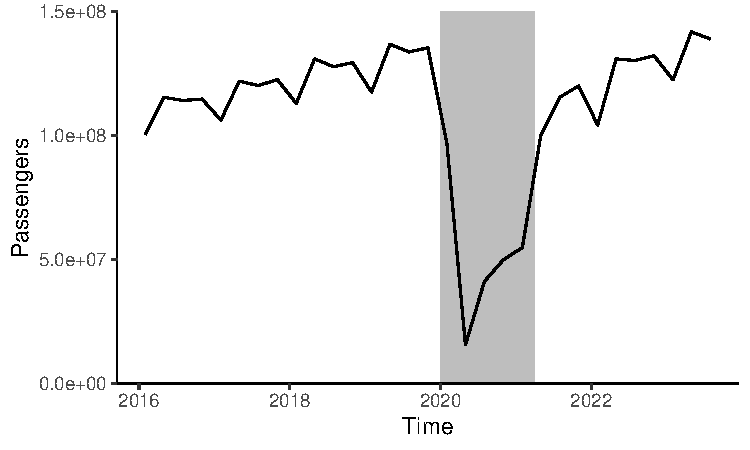
\includegraphics[width = \textwidth]{Quarterly_DB1B_Itineraries}
	\end{frame}
		
	\section{Setting}
	\begin{frame}
		\frametitle{Setting}
		\framesubtitle{United States Aviation Market}
		\begin{itemize}
			\item Post-Industry Coronavirus Changes
			\begin{itemize}
				\item Increased Tourist Travelers 
				\item Decreased Business Travelers
				\item Unclear Expectation of Change to Elasticity
			\end{itemize}
		\end{itemize} 
	\end{frame}



	\begin{frame}
		\frametitle{Setting}
		\framesubtitle{Spirit and JetBlue}
			\begin{itemize}
			\item JetBlue 
			\begin{itemize}
				\item Second (?) Largest Low-Cost Carrier
			\end{itemize}
			\item Spirit 
			\begin{itemize}
				\item Largest Ultra-Low Cost Carrier
				\item Maverick Firm Focused on Extremely Budget Focused Travelers 
			\end{itemize}
			\item Both 
			\begin{itemize}
	 		\item East Coast Focus
	 		\item Airbus A321 Fleets
			\end{itemize}
		\end{itemize} 
	\end{frame}

	\section{Data}
	\begin{frame}
		\frametitle{Data Sources}
		\begin{itemize}
			\item Airline Origin and Destination Survey (DB1B)
			\begin{itemize}
				\item 10\% Sample of Domestic Itineraries 
				\item Data on Origin, Destination, Price, Route, Carrier
			\end{itemize}
			\item Energy Information Administration Jet Fuel Spot Price
			\item Census Population Data
		\end{itemize}
	\end{frame}
	
	\begin{frame}
		\frametitle{Market, Product Definitions}
		\begin{itemize}
			\item Markets defined as Year-Quarter-Origin-Destination 
			\item Market Size is the Geometric Mean of the Population of the Origin, Destination MSA
			\item Products Further Defined by Carrier, Nonstop Status
			\begin{itemize}
				\item Connecting Product Characteristics are Weighted Average of Connecting Itineraries from a Firm
			\end{itemize}
		\end{itemize}
	\end{frame}

	
	\begin{frame}
		\frametitle{Summary Statistics}
		
	\end{frame}
	
	\section{Model and Results}
	\begin{frame}
		\frametitle{Strategy for Estimation}
	\end{frame}
	
	\begin{frame}
		\frametitle{Model of Interest}
	\end{frame}
	
	\begin{frame}
		
	\end{frame}
	
	\begin{frame}
		\frametitle{Merger Simulation}
	\end{frame}
	
	\begin{frame}
		\frametitle{Merger Simulation Results}
		
	\end{frame}
	
		\begin{frame}
		\frametitle{Merger Simulation Results: Average Market Fares}
		
	\end{frame}
	
	\begin{frame}
		\frametitle{Merger Simulation Results: Minimum Market Fares}
		
	\end{frame}
	

	
	\section{Conclusion}
	\begin{frame}
		\frametitle{Conclusion}

	\end{frame}


	\begin{frame}
		\frametitle{Thank You}
	\end{frame}

	\bibliography{airline}
	\bibliographystyle{abbrvnat.bst}
	
\end{document}


